\documentclass{article}
\usepackage{arxiv}

\usepackage{amsmath}
\usepackage[linesnumbered,ruled,vlined]{algorithm2e}
\usepackage[utf8]{inputenc}
\usepackage[english, russian]{babel}
\usepackage[T1]{fontenc}
\usepackage{url}
\usepackage{dsfont}
\usepackage{booktabs}
\usepackage{amsfonts}
\usepackage{nicefrac}
\usepackage{microtype}
\usepackage{lipsum}
\usepackage{graphicx}
\usepackage{natbib}
\usepackage{doi}

\SetKwInput{KwInput}{Input}                % Set the Input
\SetKwInput{KwOutput}{Output}              % set the Output



\title{A template for the \emph{arxiv} style}

\author{ David S.~Hippocampus\thanks{Use footnote for providing further
		information about author (webpage, alternative
		address)---\emph{not} for acknowledging funding agencies.} \\
	Department of Computer Science\\
	Cranberry-Lemon University\\
	Pittsburgh, PA 15213 \\
	\texttt{hippo@cs.cranberry-lemon.edu} \\
	%% examples of more authors
	\And
	Elias D.~Striatum \\
	Department of Electrical Engineering\\
	Mount-Sheikh University\\
	Santa Narimana, Levand \\
	\texttt{stariate@ee.mount-sheikh.edu} \\
	%% \AND
	%% Coauthor \\
	%% Affiliation \\
	%% Address \\
	%% \texttt{email} \\
	%% \And
	%% Coauthor \\
	%% Affiliation \\
	%% Address \\
	%% \texttt{email} \\
	%% \And
	%% Coauthor \\
	%% Affiliation \\
	%% Address \\
	%% \texttt{email} \\
}
\date{}

\renewcommand{\shorttitle}{\textit{arXiv} Template}

%%% Add PDF metadata to help others organize their library
%%% Once the PDF is generated, you can check the metadata with
%%% $ pdfinfo template.pdf
\hypersetup{
pdftitle={A template for the arxiv style},
pdfsubject={q-bio.NC, q-bio.QM},
pdfauthor={David S.~Hippocampus, Elias D.~Striatum},
pdfkeywords={First keyword, Second keyword, More},
}

\begin{document}
\maketitle

\begin{abstract}
	\lipsum[1]
\end{abstract}


\keywords{First keyword \and Second keyword \and More}

\section{Introduction}
\subsection{What is Schrödinger Bridge Problem?}
Let it is given two  distributions $\pi_0(x)$ and $\pi_1(y)$ (where at time 0 and 1), that describes two data distributions of  functions  $x, y\in\mathcal{C}([0,1], \mathbb{R}^d)$ at $t=0$ and time $t=1$, respectively. Also, consider:
$$\pi_1(y) \neq \int p(y|x)\pi_0(x)dx,$$
where $p(y_1|x_0)$ -- the transition density (i.e. the probability of transitioning from $x$ at time $0$ to $y$ at time $1$) under the Brownian motion. In other words, $\pi_1(y)$ differs significantly from the distribution predicted by Brownian motion. Или другими словами, мы не ограничиваем жестко броуновское движение, чтобы оно приходило во второе распределение \par 
% The Schrödinger Bridge problem considers the finding of most likely stochastic process that transforms the distribution $\pi_0(x)$ at time $0$ to $\pi_1(y)$ at time $1$ and is closer in information-theoretic sense.
Основная мотивация Schrödinger Bridge Problem посторить стохостический процесс между $\pi_0(x)$ and $\pi_1(y)$. Для этого рассмотрим некоторый набор броуновских движений (винеровских процессов) \{$x_i(t)\}^N_{i=1}$, где каждый элемент данного множества принадлежит множеству всех функций $\mathcal{C}([0,1], \mathbb{R}^d)$, т.е. $x:[0,1]\rightarrow \mathbb{R}^d$.\par 
Также зададим новое понятие Path measure. Path measure is a weak solution for given SDE, i.e. a stochastic process. Weak solution is a terminology for a solution of an SDE, that does not take into account an initial value problem and has the freedom of specifying its probability space. В дискретном случае path measure определяется слудющим образом:


\begin{equation} \label{eq1}   
    \hat{\mathbb{W}}(A)=\frac{1}{N}\sum_{i=1}^N\mathds{1}\left(x_i(t)\in A\right), A\in \mathcal{B}(\mathbb{R}^d)^{[0,1]}
\end{equation}


Однако, данное определение не гарантирует, что at time $0$ to $y$ at time $1$, распределение будет совпадать с заданным. Поэтому теперь ограничим path measure $\hat{\mathbb{W}}$:
\begin{equation} \label{eq2}
    P\left(\hat{\mathbb{W}} \in \mathcal{D}(\pi_0, \pi_1)\right)=1
\end{equation}
Т.е. вероятность того, что данный path measure принадлежит множеству всех path measures with two prescribed marginals равнялась единице. Из теоремы Санова, изветстно, что асимтотически данная вероятность стремится к следующему выражению:
\begin{equation} \label{eq3}
    P\left(\hat{\mathbb{W}} \in \mathcal{D}(\pi_0, \pi_1)\right) \xrightarrow{N\rightarrow \infty} \exp\left(-N\inf_{\mathbb{Q} \in \mathcal{D}(\pi_0, \pi_1)}\mathbb{KL(Q||W})\right)
\end{equation}

Таким образом, для того, чтобы выбполнялось условие \ref{eq2} требуется, чтобы $\mathbb{KL}$ дивергенция была минимальной.
Overall, the Schrödinger bridge provides us with a theoretically-grounded mechanism for mapping between two distribution to solve such problems like unsupervised domain adaptation and also gives the with the probability of this stochastic evolution, thus allowing us to compare two datasets/distributions which can be useful for hypothesis testing and semantic similarity
So, speaking formally, there are two approaches to problem setting, dynamic and static.
\subsection{Dynamic Schrödinger Bridge Problem}
Данная постановка задачи выходит из теоремы \ref{eq3} . In this approach is minimizing of KL divergence between two \textit{path measures} $\mathbb{Q}$ and $\mathbb{W}^\gamma$, path measures of our desired process and prior Wiener process with drift coefficient $\sqrt\gamma$.
\begin{equation}
    \hat{\mathbb{Q}} = \arg\min_{\mathbb{Q}\in \mathcal{D}(\pi_0, \pi_1)} \mathbb{KL(Q||W}^\gamma)
\end{equation}

вывод в статик
\subsection{Static Schrödinger Bridge Problem}
In this approach is minimizing of $\mathbb{KL}$ divergence between two joint distributions $q(x,y)$ and $p^{\mathbb{W}^\gamma}(x,y)$

$$\left\{ \begin{array}{c}
\hat q(x,y) = \arg\min_{q(x,y)} KL(q(x,y)||p^{\mathbb{W}^\gamma}(x,y)), \\
\pi_0(x) = \int q(x,y)dy, \\
\pi_1(y) = \int q(x,y)dx
\end{array}\right.$$
where $q(x,y)$ is a joint distribution which is closest to the Brownian-motion prior subject to marginal constraints (between PDF at time 0 and 1)
\subsection{Schrödinger System}
Applying Lagrangian on static SBP we get
\begin{equation}
    L(q, \lambda, \mu) = KL(q(x,y)||p^{\mathbb{W}^\gamma}(x,y)) + \int \lambda(x)\left(\int q(x, y)dy - \pi_0(x)\right)dx + \int \mu(y)\left(\int q(x, y)dy - \pi_1(y)\right)dy
\end{equation}
Предполагая, что $p^{\mathbb{W}^\gamma}(x,y) = p_0^{\mathbb{W}^\gamma}(x)p^{\mathbb{W}^\gamma}(y|x)$, где $p_0^{\mathbb{W}^\gamma}(x)$ может быть любым, а $p^{\mathbb{W}^\gamma}(y|x)=\mathcal{N}(y|x, \gamma I_d)$ (это выходит из свойств Винеревского процесса).  Теперь приравняем нулю $ \frac{\partial L(q, \lambda, \mu)}{\partial q(x,y)}$
\begin{equation}
    q^*(x, y) = \exp{(\ln{p^{\mathbb{W}^\gamma}(x,y)} - \lambda(x) - 1)}p^{\mathbb{W}^\gamma}(y|x)\exp{(-\mu(y))}
\end{equation}
Теперь положив, что  $\hat\phi_0(x) = \exp{(\ln{p^{\mathbb{W}^\gamma}(x,y)} - \lambda(x) - 1)}$ и $\phi_1(y) = \exp{(-\mu(y))}$ получаем
\begin{equation}\label{eq7}
    q^*(x, y) = \hat\phi_0(x)p^{\mathbb{W}^\gamma}(y|x)\phi_1(y)
\end{equation}
маргинализуя данное распределение по $x$ или $y$ получим
\begin{equation}
\begin{split}
    \pi_0(x) = \hat\phi_0(x)\phi_0(x) \\
    \pi_1(y) = \phi_1(y)\hat\phi_1(y)
\end{split}
\end{equation}
где  $\phi_0(x) = \int\phi_1(y)p^{\mathbb{W}^\gamma}(y|x)dy$, а $\hat\phi_1(y) = \int\hat\phi_0(x)p^{\mathbb{W}^\gamma}(y|x)dx$
\subsection{Iteration Proportional Fitting (IPF)}
One of the oldest algorithms for solving Schrödinger Bridge Problem is Fortret's algorithm (1940).

\begin{algorithm}
\caption{Fortret's Algorithm}\label{alg:fortret}
\KwInput{$\pi_0(x)$, $\pi_1(y)$, $p(y|x)$}
\KwOutput{$\hat\phi^{(i)}_0(x)$, $\phi^{(i)}_1(y)$}
Initialize $\phi_0^{(0)}(x)$ s.t. $\phi_0^{(0)}(x)<<\pi_0(x)$\;
\While{not converged}{
    $\hat\phi_0^{(i)}(x):=\frac{\pi_0(x)}{\phi_0^{(i)}(x)}$\;
   $\hat\phi_1^{(i)}(y):=\int p(y|x)\hat\phi_0^{(i)}(x)dx$\;
    $\phi_1^{(i)}(y):=\frac{\pi_1(y)}{\hat\phi_1^{(i)}(y)}$\;
    $\hat\phi_1^{(i+1)}(x):=\int p(y|x)\phi_1^{(i)}(y)dy$\;
    $i:=i+1$\;
   }
\end{algorithm}

\section{Related works}
\label{sec:headings}
\subsection{Diffusion Schrodinger Bridge Matching (DSBM)}
Authors proposed new method of solving SBP in dynamic way using Iterative Markovian Fitting
\subsection{Diffusion Schrodinger Bridge with Applications to Score-Based Generative Modeling}
Authors proposed using SBP in dynamic way to build generative model


\section{Examples of citations, figures, tables, references}
\label{sec:others}

\subsection{Citations}
Citations use \verb+natbib+. The documentation may be found at
\begin{center}
	\url{http://mirrors.ctan.org/macros/latex/contrib/natbib/natnotes.pdf}
\end{center}

Here is an example usage of the two main commands (\verb+citet+ and \verb+citep+): Some people thought a thing \citep{kour2014real, hadash2018estimate} but other people thought something else \citep{kour2014fast}. Many people have speculated that if we knew exactly why \citet{kour2014fast} thought this\dots

\subsection{Figures}
\lipsum[10]
See Figure \ref{fig:fig1}. Here is how you add footnotes. \footnote{Sample of the first footnote.}
\lipsum[11]

\begin{figure}
	\centering
	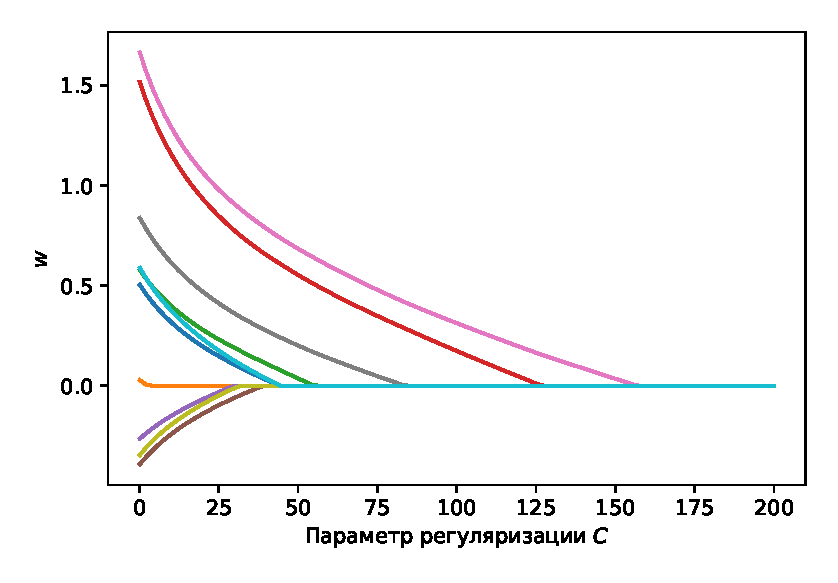
\includegraphics[width=0.5\textwidth]{../figures/log_reg_cs_exp.eps}
	\caption{Sample figure caption.}
	\label{fig:fig1}
\end{figure}

\subsection{Tables}
See awesome Table~\ref{tab:table}.

The documentation for \verb+booktabs+ (`Publication quality tables in LaTeX') is available from:
\begin{center}
	\url{https://www.ctan.org/pkg/booktabs}
\end{center}


\begin{table}
	\caption{Sample table title}
	\centering
	\begin{tabular}{lll}
		\toprule
		\multicolumn{2}{c}{Part}                   \\
		\cmidrule(r){1-2}
		Name     & Description     & Size ($\mu$m) \\
		\midrule
		Dendrite & Input terminal  & $\sim$100     \\
		Axon     & Output terminal & $\sim$10      \\
		Soma     & Cell body       & up to $10^6$  \\
		\bottomrule
	\end{tabular}
	\label{tab:table}
\end{table}

\subsection{Lists}
\begin{itemize}
	\item Lorem ipsum dolor sit amet
	\item consectetur adipiscing elit.
	\item Aliquam dignissim blandit est, in dictum tortor gravida eget. In ac rutrum magna.
\end{itemize}


\bibliographystyle{unsrtnat}
\bibliography{references}

\end{document}